The general notion of an elliptic curve shall be the centre of
focus for this thesis. One might define an Elliptic Curve as follows.
\begin{definition} \label{def:ellipticCurve}
  Let $f(x)$ be a 3rd degree monic polynomial having distinct roots.
  An Elliptic Curve is a curve
  \[ E: y^2 = f(x). \]
  If $K$ is a field, we denote for a given Elliptic Curve
  \[ E(K) := \left\{ (x,y) \in K \times K : y^2 = f(x) \right\} \cup \{\mathcal{O}\}, \]
  where $\mathcal{O}$ is the point at infinity.
\end{definition}
Since we are talking about an Elliptic \textit{Curve} it is tempting
to look at a case where $K$ allows us to draw a continuous line to
depict an Elliptic Curve.
\begin{example} \label{ex:curveExamplesContinuous}
  Take $K = \mathbb{R}$, $f(x) = x^3 + px^2 + 1$, where we let $r \in \left\{ -2,\dots, 3 \right\}$.
  This yields a sequence of Elliptic Curves $E_p$, we used
  python to depict these curves on $[-5, 5] \times [-5, 5]$.
  \begin{figure}[H]
    \centering
    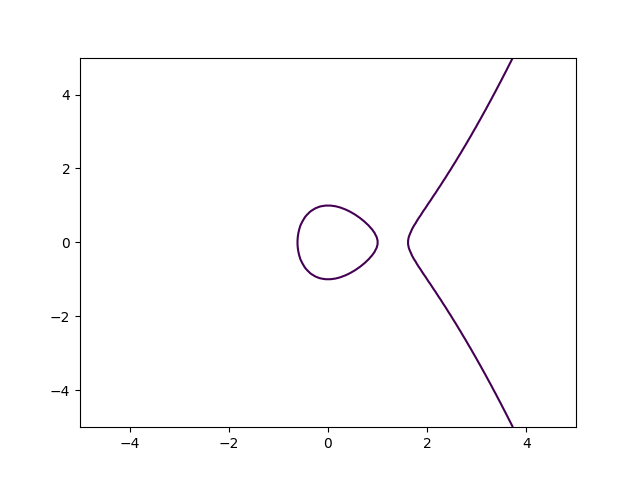
\includegraphics[width=0.3\linewidth]{ellipticCurves/example1p-2.png}
    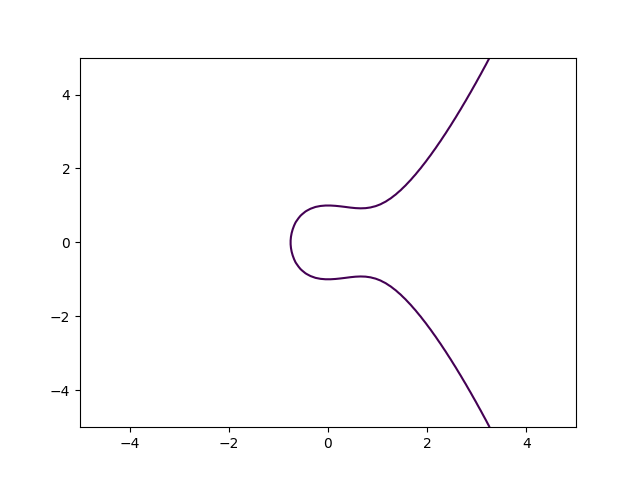
\includegraphics[width=0.3\linewidth]{ellipticCurves/example1p-1.png}
    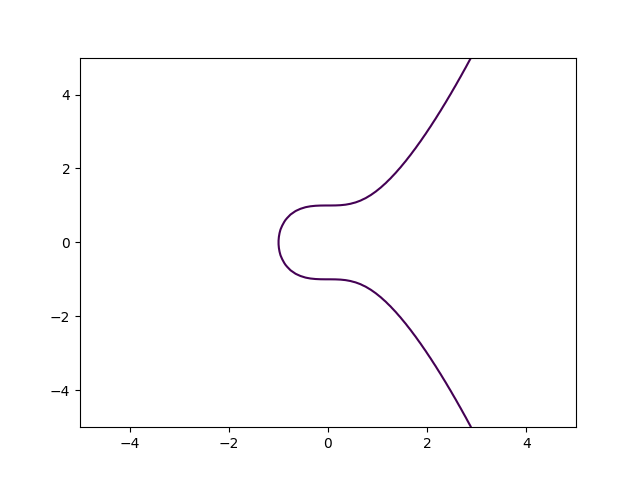
\includegraphics[width=0.3\linewidth]{ellipticCurves/example1p0.png}
    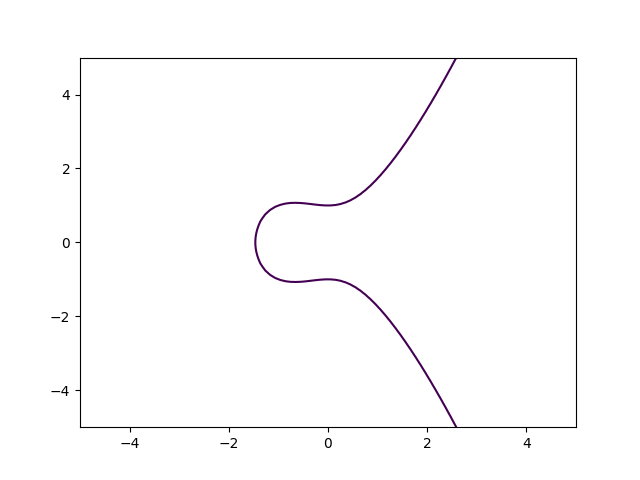
\includegraphics[width=0.3\linewidth]{ellipticCurves/example1p1.png}
    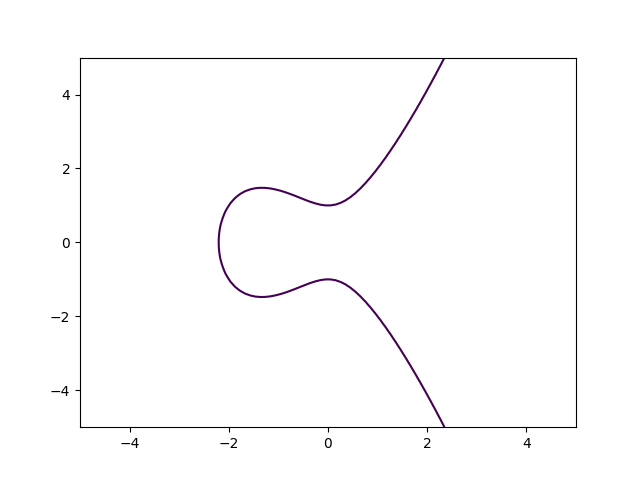
\includegraphics[width=0.3\linewidth]{ellipticCurves/example1p2.png}
    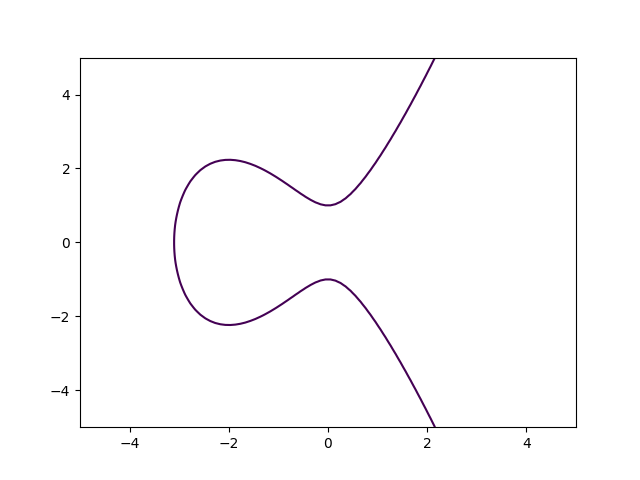
\includegraphics[width=0.3\linewidth]{ellipticCurves/example1p3.png}
    \caption{The curves $y^2 = x^3 + px^2 + 1$ for $p \in \{-2, \dots, 3\}$.}%
    \label{fig:curvesExamples}
  \end{figure}
\end{example}
It should be noted that an Elliptic Curve is not always a curve
in the Calculus sense, but may also consist of a series of seemingly
random points. As is illustrated in the following example.
\begin{example} \label{ex:curveExamplesFinite}
  Let $K = \mathbb{F}_{p}$, $p \equiv 3 \mod 4$ a prime and $f(x) = x^3 + nx$
  where $\gcd(n, p) = 1$.
  To find $E(\mathbb{F}_p)$ we wish to find when
  $x^3 + nx$ is a square modulo $p$.
  Note that $-1$ is not a square, since the Legendre Symbol equals
  \begin{align*}
    \left( \frac{-1}{p}  \right) = (-1)^{\frac{p-1}{2} } = (-1)^{\frac{3 + 4k - 1}{2} } = (-1)^{1 + 2 k} = -1.
  \end{align*}
  Fix some $a \in \mathbb{F}_p$ which is not a root of $f$,
  then
  \begin{align*}
    \legendre{a^3+na}{p}\legendre{(-a)^3+n(-a)}{p}
    = \legendre{a}{p}^2 \legendre{-1}{p}\legendre{a^3+na}{p}^2
    = -1.
  \end{align*}
  Hence precisely one of $f(a)$ and $f(-a)$ is a square.
  So for half of all residue classes $x$ we can find two points $(\sqrt{f(\pm x)},x)$ and
  $(-\sqrt{f(\pm x)}, x)$ on the curve. Hence including the point at infinity
  we have
  \begin{align*}
    \# E(\mathbb{F}_p) = p + 1.
  \end{align*}
  For instance when $p = 7$ we have
  \begin{align*}
    E(\mathbb{F}_p) = \left\{ \mathcal{O}, (0, 0), (3, 1), (4, 1), (3, 3), (4, 3), (2, 5), (5, 5) \right\}.
  \end{align*}
\end{example}
The main reason we are interested in Elliptic Curves is that $E(K)$ is an Abelian Group.
In the case that $K = \mathbb{Q}$ there is a geometric interpretation of what
this means, which uses only calculus.

\subsection{Elliptic Curves over the Rationals}
\label{sub:elliptic_curves_over_the_rationals}
We take $E: y^2 = f(x)$ to be an Elliptic Curve over $\mathbb{Q}$.
As an example of such a curve we take $f(x) = x^3 - 6x + 9$.
Say we take two points on this curve, say $(-3, 0)$ and $(1,2)$.
Then note we can draw a line through both of these points and it intersects
the curve at a 3rd point.
\begin{figure}[H]
  \centering
  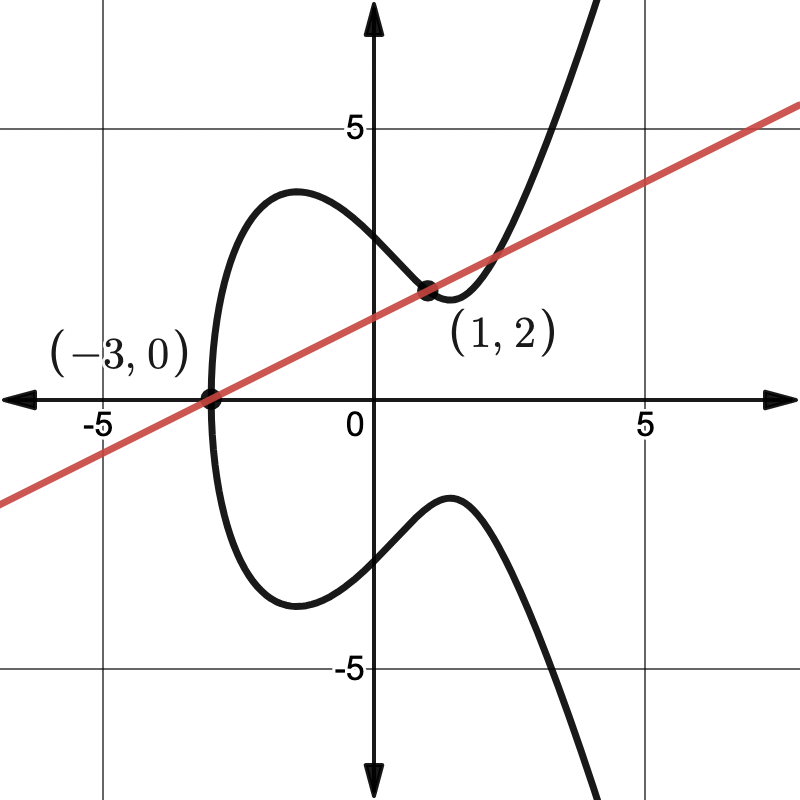
\includegraphics[width=0.5\linewidth]{ellipticCurves/ellipticCurveImage1.png}
  \caption{Two points on $y^2 = f(x)$ }%
  \label{fig:ellipticCurves/ellipticCurveImage1}
\end{figure}
In fact, barring a few exceptions, we can use this method to obtain
a 3rd point when we know two points on the curve.

When we have two distinct points $(x_1,y_1), (x_2,y_2) \in E(\mathbb{Q})$ we can use
calculus to find a line through both, namely the line
\begin{align*}
  y = \frac{y_2 - y_1}{x_2 - x_1} (x - x_1) + y_1.
\end{align*}
Note that this line does not intersect the curve in a 3rd point in $\mathbb{Q}$
when $y_1 = y_2$. Barring this case though, we find via a straightforward computation
that
\begin{equation} \label{eq:3rdPoint}
  x_3 = \left[ \frac{y_2 - y_1}{x_2 - x_1}  \right]^2 - (x_1 + x_2), \qquad y_3 = y_1 + \frac{y_2 - y_1}{x_2 - x_1} (x_3 - x_1)
\end{equation}
is also a point on this curve.

If the points are not distinct, then \cite[chapter 1.4]{silvermanRationalPoints}
describes how we can similarly use the tangent line, which also leads
to a point with coordinates in $\mathbb{Q}$.
\emptyline
At this point it is tempting to define a group law
by mapping $*: ((x_1,y_1), (x_2, y_2)) \mapsto (x_3, y_3)$. Sadly this
is not associative.

\begin{counterexample} \label{counterexample:notAssociative}
  Let $E: y^2 = f(x)$ as above over $\mathbb{Q}$.
  We find the line through $(-3, 0), (1,2)$ to be
  \begin{align*}
    y = \frac{x}{2} + \frac{3}{2}.
  \end{align*}
  and we solve
  \begin{align*}
    \left(\frac{x}{2} + \frac{3}{2}\right)^2 = x^3 - 6x + 9
  \end{align*}
  which has a solution $9/4$, giving a 3rd point $(9/4, 9/8 + 3/2)$,
  which we set $(-3, 0) * (1, 2)$.  Now similarly we compute $((-3, 0) * (1,2)) * (-1.414, 3.828) = (-0.727,3.602)$.

  On the other hand, we find
  $ (1,2) * (-1.414, 3.828) = (0.9879, 2.0092) $
  and thus so we find $(-3, 0) * (0.9879, 2.0092) = (2.266, 2.6531)$
\end{counterexample}

\subsubsection{The Group law}%
\label{ssub:the_group_law}
Luckily a small modification of $*$ does yield an associative operation,
namely when we take the 3rd point of intersection, and take its
antipode in the $y$ axis.
\begin{figure}[H]
  \centering
  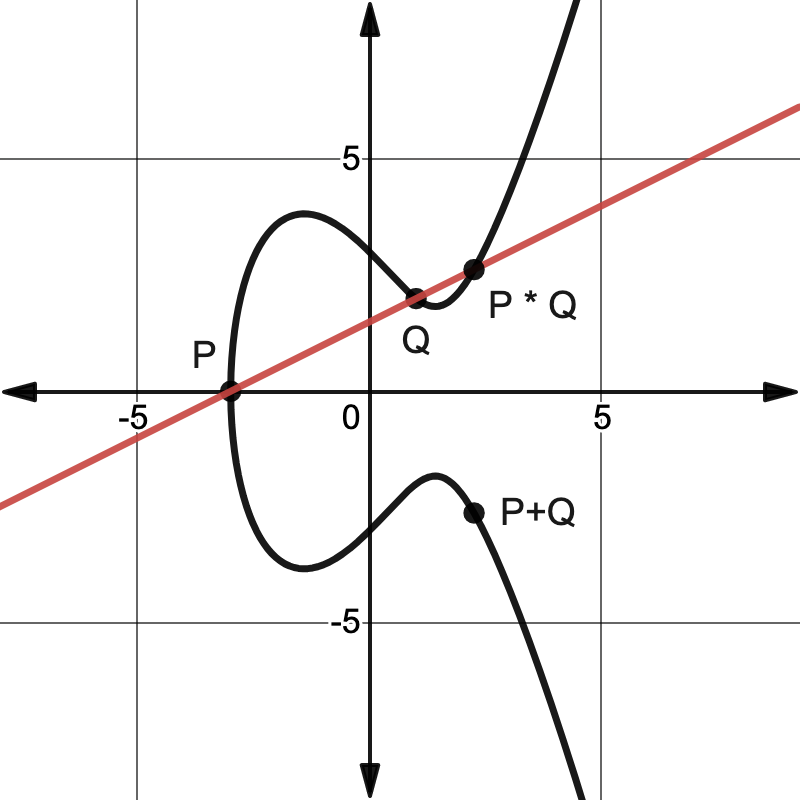
\includegraphics[width=0.5\linewidth]{ellipticCurves/ellipticCurveImage2.png}
  \caption{Depiction of the group law}%
  \label{fig:ellipticCurves/ellipticCurveImage2}
\end{figure}
This still leaves a number of edge cases.
For instance, when two points are antipodes
there is not going to be a 3rd point of intersection in $\mathbb{Q}^2$.
Luckily we have a point at infinity, which we will define
to be the sum of two antipodes.

After this motivation we introduce the following definition,
which is used by \cite[section 1.4]{silvermanRationalPoints}.
\begin{definition} \label{def:groupLaw}
  Let $P = (x_1, y_1), Q = (x_2, y_2)$ be points on an Elliptic curve $y^2 = x^3 - ax - b$, define an operation $+_E$ as follows.
  \begin{enumerate}
    \item If $P \neq Q$ and $x_1 = x_2$ then $P +_E Q = \mathcal{O}$.
    \item If $P = Q$ and $y_1 = 0$ then $P +_E Q = \mathcal{O}$
  \end{enumerate}
  If neither of these are the case we define $\lambda$ and $\nu$ as follows.
  \begin{enumerate}
    \item if $P \neq Q$ and $x_1 \neq x_2$
      then
      \[ \lambda = \frac{y_2 - y_1}{x_2 - x_1},\qquad \nu = \frac{y_1x_2 - y_2 x_1}{x_2 - x_1}.\]
    \item If $P = Q$ and $y_1 \neq 0$ then
      \[ \lambda = \frac{3x_1^2 + a}{2y_1},\qquad \nu = \frac{-x_1^3 + ax_1 + 2b}{2y_1} \]
  \end{enumerate}
  then
  \[ P +_E Q = (\lambda^2 - x_1 - x_2, -\lambda^3 + \lambda (x_1 + x_2) - \nu). \]
  When it is clear from context what the curve is, we will write $+$ instead of $+_E$.
\end{definition}
So we have a set, together with a binary operation. This
motivates the following theorem.
\begin{theorem}
  Let $E: y^2 = f(x)$ be an elliptic curve. Then
  $(E(\mathbb{Q}), +_E, \mathcal{O})$ is an Abelian Group.
\end{theorem}
\begin{proof}
  By construction, we have that $+_E: E(\mathbb{Q}) \times E(\mathbb{Q}) \to E(\mathbb{Q})$
  is well defined. Namely, it is clear from equation \ref{eq:3rdPoint}
  that when $P, Q \in E(\mathbb{Q})$, then also $P * Q \in E(\mathbb{Q})$.
  Consequently, the projection in the $y-axis$ is also in $E(\mathbb{Q})$.

  Moreover, if we have a line $y = ax + b$ through $P, Q \in E(\mathbb{Q})$, then
  this yields an equality
  \begin{align*}
    \left(\frac{y_2 - y_1}{x_2 - x_1} (x - x_1) + y_1\right)^2 = x^3 + px^2 + qx + r
  \end{align*}
  Which yields a root finding problem $\tilde{f}(x) = 0$.
  We know that we can factor $\tilde{f}(x) = (x - x_1)(x - x_2)(x - A)$,
  for some $A$. We argue $A$ must be rational, since if $A \notin \mathbb{Q}$,
  then we would have
  \begin{align*}
    \tilde{f}(x) = -A x_1 x_2 + A x_1 x + A x_2 x - A x^2 + x_1 x_2 x - x_1 x^2 - x_2 x^2 + x^3
  \end{align*}
  not having rational coefficients. But clearly $\tilde{f}$ must have rational coefficients,
  we conclude $A$ is the $x$ coordinate of a 3rd point of intersection, and moreover
  there cannot be any more factors, so there are precisely 3 points of intersection.
  So indeed $+_E$ is well-defined.

  It should also be clear that $+_E$ is commutative, since $P +_E Q$ and $Q +_E P$ would
  yield the same 3rd point of intersection.

  Inverses are also straightforward: we think of $\mathcal{O}$ of sitting at infinity,
  so the line through a point and its antipode (which may be the point itself if we are
  talking about points like $(-3, 0)$ as in \ref{fig:ellipticCurves/ellipticCurveImage1})
  will only intersect at infinity.

  The proof of $+_E$ being associative can be found in \cite[section 2.4]{washingtonElliptic}
\end{proof}
We shall from now on just denote $E(\mathbb{Q})$ to indicate this group.
\begin{example}
  The curve $E: y^2 = x^3 - 6x^2 -9x + 1$ over $\mathbb{Q}$ is
  finitely generated.
  Using SageMath we found
  \begin{python}
sage: E = EllipticCurve([0,-6,0,-9,1]); E
Elliptic Curve defined by y^2 = x^3 - 6*x^2 - 9*x + 1 over Rational Field
sage: E.gens()
[(0 : 1 : 1), (240 : 3671 : 1)]
sage: E.rank()
2
  \end{python}
  Hence using the structure theorem we find there is some Abelian group $A$
  such that
  \begin{align*}
    E(\mathbb{Q}) \simeq \mathbb{Z}^2 \times A
  \end{align*}

\end{example}

\subsection{Elliptic Curves over an Arbitrary Field}%
\label{sub:elliptic_curves_over_an_arbitrary_field}
In an arbitrary field we can define $+$ analogously to definition \ref{def:groupLaw}.
And again we have
\begin{theorem}
  Let $K$ be a field, and $E: y^2 = f(x)$ an elliptic curve.
  Then $(E(K), +_E, \mathcal{O})$ is an Abelian Group.
\end{theorem}
This yields the following
\begin{example} \label{ex:curveOfPplus1}
  Let $p$ be a prime and $E: y^2 = f(x)$ an elliptic curve.
  For any finite field $\mathbb{F}_{p^n}$ we surely have
  $E(\mathbb{F}_{p^n})$ is finite. So by the structure theorem
  \cite[theorem 2.8]{sergeLangAlgebra}
  there exist finitely many $a_i \in \mathbb{N}_0$
  such that
  \begin{align*}
    E(\mathbb{F}_{p^{n}}) \simeq \mathbb{Z}/a_0\mathbb{Z} \times \dots \times \mathbb{Z}/a_{k}\mathbb{Z}.
  \end{align*}
  In example \ref{ex:curveExamplesFinite} we found that for
  $p \equiv 3 \mod 4$ a curve $E: y^2 = x^3 + nx$ has $\# E(\mathbb{F}_p) = p + 1$.

  When $p = 43$ we have $\#E(\mathbb{F}_{43}) = 44 = 2^2 \cdot 11$,
  hence the only two Abelian groups of this order are
  $\mathbb{Z}/11\mathbb{Z} \times \mathbb{Z}/4\mathbb{Z}$ and
  $\mathbb{Z}/11\mathbb{Z} \times \mathbb{Z}/2\mathbb{Z} \times \mathbb{Z}/2\mathbb{Z}$.
  It can be verified that $(42, 27)$ is a point of order 4, so
  \begin{align*}
    E(\mathbb{F}_{43}) \simeq \mathbb{Z}/11\mathbb{Z} \times \mathbb{Z}/4\mathbb{Z} \simeq \mathbb{Z}/44\mathbb{Z}.
  \end{align*}
  Numerically, it appears that when $n$ is a square these groups
  are always cyclic.
\end{example}
There is a well-known class of primes which have some nice behaviour over
these curves
\begin{example} \label{ex:mersenneCurve}
  Let $E: y^2 = f(x)$ over $\mathbb{F}_{p}$ be as in example \ref{ex:curveOfPplus1}.
  There is the famous class of Mersenne Primes, which are primes of
  the form $2^p - 1$, where $p$ is a prime. An efficient
  algorithm exists to determine the primality of these numbers
  \cite{bruceLLTest}
\end{example}

\subsection{Isogenies}%
\label{sub:isogenies}
Since we know that an Elliptic Curve $E: y^2 = f(x)$ over a
field $K$ has an associated group $E(K)$, it is natural
to speak about group homomorphisms between these groups.
This leads us to the following definition.
\begin{definition} \label{def:isogeny}
  Let $E_1, E_2$ be Elliptic Curves over a field $K$.
  An isogeny $\varphi: E_1(K) \to E_2(K)$ is a rational function
  that is also a group homomorphism.
\end{definition}
The astute reader might notice that this definition is
over-engineered, as one can prove that any rational function
$\varphi: E_1(K) \to E_2(K)$ satisfying $\varphi: \mathcal{O} \mapsto \mathcal{O}$
would automatically be a group homomorphism. And this is indeed what
Silverman proves \cite[Theorem III.4.8]{silvermanRationalPoints}
the following theorem.
\begin{theorem} \label{thm:rationalMapsAreIsogeny}
  Let $E_1, E_2$ be Elliptic Curves over a field $K$
  and $\varphi: E_1(K) \to E_2(K)$ be rational maps
  such that $\varphi(\mathcal{O}) = \mathcal{O}$,
  then $\varphi$ is a group homomorphism.
\end{theorem}
Below we shall go into some examples
that shall come in useful later.
\begin{example} \label{ex:multiplicationIsogeny}
  Fix some $n \in \mathbb{N}$ then $[n]: P \mapsto nP$ is an isogeny, since
  it is clearly a rational function, and it is also a homomorphism
  of groups as by definition $n \mathcal{O} = \mathcal{O}$. And since
  the group of rational points on an elliptic curve is abelian
  \[ nA + nB = A + \dots A + B + \dots B = A + B + \dots + A + B = n(A+B). \]
\end{example}
The following example is the subject of \cite[chapter 2.2]{moniqueThesis}
\begin{example} \label{eq:dualIsogenies}
  Let $A, B \in \mathbb{Q}$ and $\bar{A} = -27A, \bar{B} = 4A + 27B$
  \begin{align*}
    E: y^2 = x^3 + A(x - B)^2, \qquad \bar{E} \eta^2 = \xi^3 + \bar{A} (\xi - \bar{B})^2
  \end{align*}
  be Elliptic Curves, we define the map
  \[ \Phi_{X, Y}: (x, y) \mapsto (\xi, \eta), \]
  where
  \begin{align*}
    \xi &=  \frac{9}{x^2} \left( 2y^2 + 2XY^2 - x^3 - \frac{2}{3} X x^2  \right), \\
    \eta &= \frac{27y}{x^3} \left( -4XYx + 8XY^2 - x^3 \right).
  \end{align*}
  If we define $\Phi_{X, Y}: \mathcal{O} \mapsto \mathcal{O}$ then by
  theorem \ref{thm:rationalMapsAreIsogeny} it follows
  that $\Phi_{X, Y}$ is an isogeny.
  If we apply the map $\Phi_{\bar{A}, \bar{B}} \circ \Phi_{A, B}$
  we obtain the curve
  \begin{align*}
    C: y^2 = x^3 + 3^{6}A(x - 3^6 B)^2.
  \end{align*}
  The change of coordinates
  \begin{align*}
    (x, y) \mapsto (3^6 x, 3^9 y)
  \end{align*}
  gives
  \begin{align*}
    3^{18}y = 3^{18}x^2 + 3^{18}A(x - B)^2
  \end{align*}
  which is the equation of $E$ multiplied by $3^{18}$.
  In conclusion the following diagram commutes
  \begin{equation*}
  \begin{tikzcd}
    E(\mathbb{Q}) \ar[rr, bend left, "\begin{bmatrix}3\end{bmatrix}"] \ar[r, "\Phi_{A, B}"] & \bar{E}(\mathbb{Q}) \ar[r, "\Phi_{\bar{A}, \bar{B}}"] & C(\mathbb{Q})
  \end{tikzcd}
  \end{equation*}

\end{example}
